\documentclass[1p]{elsarticle_modified}
%\bibliographystyle{elsarticle-num}

%\usepackage[colorlinks]{hyperref}
%\usepackage{abbrmath_seonhwa} %\Abb, \Ascr, \Acal ,\Abf, \Afrak
\usepackage{amsfonts}
\usepackage{amssymb}
\usepackage{amsmath}
\usepackage{amsthm}
\usepackage{scalefnt}
\usepackage{amsbsy}
\usepackage{kotex}
\usepackage{caption}
\usepackage{subfig}
\usepackage{color}
\usepackage{graphicx}
\usepackage{xcolor} %% white, black, red, green, blue, cyan, magenta, yellow
\usepackage{float}
\usepackage{setspace}
\usepackage{hyperref}

\usepackage{tikz}
\usetikzlibrary{arrows}

\usepackage{multirow}
\usepackage{array} % fixed length table
\usepackage{hhline}

%%%%%%%%%%%%%%%%%%%%%
\makeatletter
\renewcommand*\env@matrix[1][\arraystretch]{%
	\edef\arraystretch{#1}%
	\hskip -\arraycolsep
	\let\@ifnextchar\new@ifnextchar
	\array{*\c@MaxMatrixCols c}}
\makeatother %https://tex.stackexchange.com/questions/14071/how-can-i-increase-the-line-spacing-in-a-matrix
%%%%%%%%%%%%%%%

\usepackage[normalem]{ulem}

\newcommand{\msout}[1]{\ifmmode\text{\sout{\ensuremath{#1}}}\else\sout{#1}\fi}
%SOURCE: \msout is \stkout macro in https://tex.stackexchange.com/questions/20609/strikeout-in-math-mode

\newcommand{\cancel}[1]{
	\ifmmode
	{\color{red}\msout{#1}}
	\else
	{\color{red}\sout{#1}}
	\fi
}

\newcommand{\add}[1]{
	{\color{blue}\uwave{#1}}
}

\newcommand{\replace}[2]{
	\ifmmode
	{\color{red}\msout{#1}}{\color{blue}\uwave{#2}}
	\else
	{\color{red}\sout{#1}}{\color{blue}\uwave{#2}}
	\fi
}

\newcommand{\Sol}{\mathcal{S}} %segment
\newcommand{\D}{D} %diagram
\newcommand{\A}{\mathcal{A}} %arc


%%%%%%%%%%%%%%%%%%%%%%%%%%%%%5 test

\def\sl{\operatorname{\textup{SL}}(2,\Cbb)}
\def\psl{\operatorname{\textup{PSL}}(2,\Cbb)}
\def\quan{\mkern 1mu \triangleright \mkern 1mu}

\theoremstyle{definition}
\newtheorem{thm}{Theorem}[section]
\newtheorem{prop}[thm]{Proposition}
\newtheorem{lem}[thm]{Lemma}
\newtheorem{ques}[thm]{Question}
\newtheorem{cor}[thm]{Corollary}
\newtheorem{defn}[thm]{Definition}
\newtheorem{exam}[thm]{Example}
\newtheorem{rmk}[thm]{Remark}
\newtheorem{alg}[thm]{Algorithm}

\newcommand{\I}{\sqrt{-1}}
\begin{document}

%\begin{frontmatter}
%
%\title{Boundary parabolic representations of knots up to 8 crossings}
%
%%% Group authors per affiliation:
%\author{Yunhi Cho} 
%\address{Department of Mathematics, University of Seoul, Seoul, Korea}
%\ead{yhcho@uos.ac.kr}
%
%
%\author{Seonhwa Kim} %\fnref{s_kim}}
%\address{Center for Geometry and Physics, Institute for Basic Science, Pohang, 37673, Korea}
%\ead{ryeona17@ibs.re.kr}
%
%\author{Hyuk Kim}
%\address{Department of Mathematical Sciences, Seoul National University, Seoul 08826, Korea}
%\ead{hyukkim@snu.ac.kr}
%
%\author{Seokbeom Yoon}
%\address{Department of Mathematical Sciences, Seoul National University, Seoul, 08826,  Korea}
%\ead{sbyoon15@snu.ac.kr}
%
%\begin{abstract}
%We find all boundary parabolic representation of knots up to 8 crossings.
%
%\end{abstract}
%\begin{keyword}
%    \MSC[2010] 57M25 
%\end{keyword}
%
%\end{frontmatter}

%\linenumbers
%\tableofcontents
%
\newcommand\colored[1]{\textcolor{white}{\rule[-0.35ex]{0.8em}{1.4ex}}\kern-0.8em\color{red} #1}%
%\newcommand\colored[1]{\textcolor{white}{ #1}\kern-2.17ex	\textcolor{white}{ #1}\kern-1.81ex	\textcolor{white}{ #1}\kern-2.15ex\color{red}#1	}

{\Large $\underline{12n_{0024}~(K12n_{0024})}$}

\setlength{\tabcolsep}{10pt}
\renewcommand{\arraystretch}{1.6}
\vspace{1cm}\begin{tabular}{m{100pt}>{\centering\arraybackslash}m{274pt}}
\multirow{5}{120pt}{
	\centering
	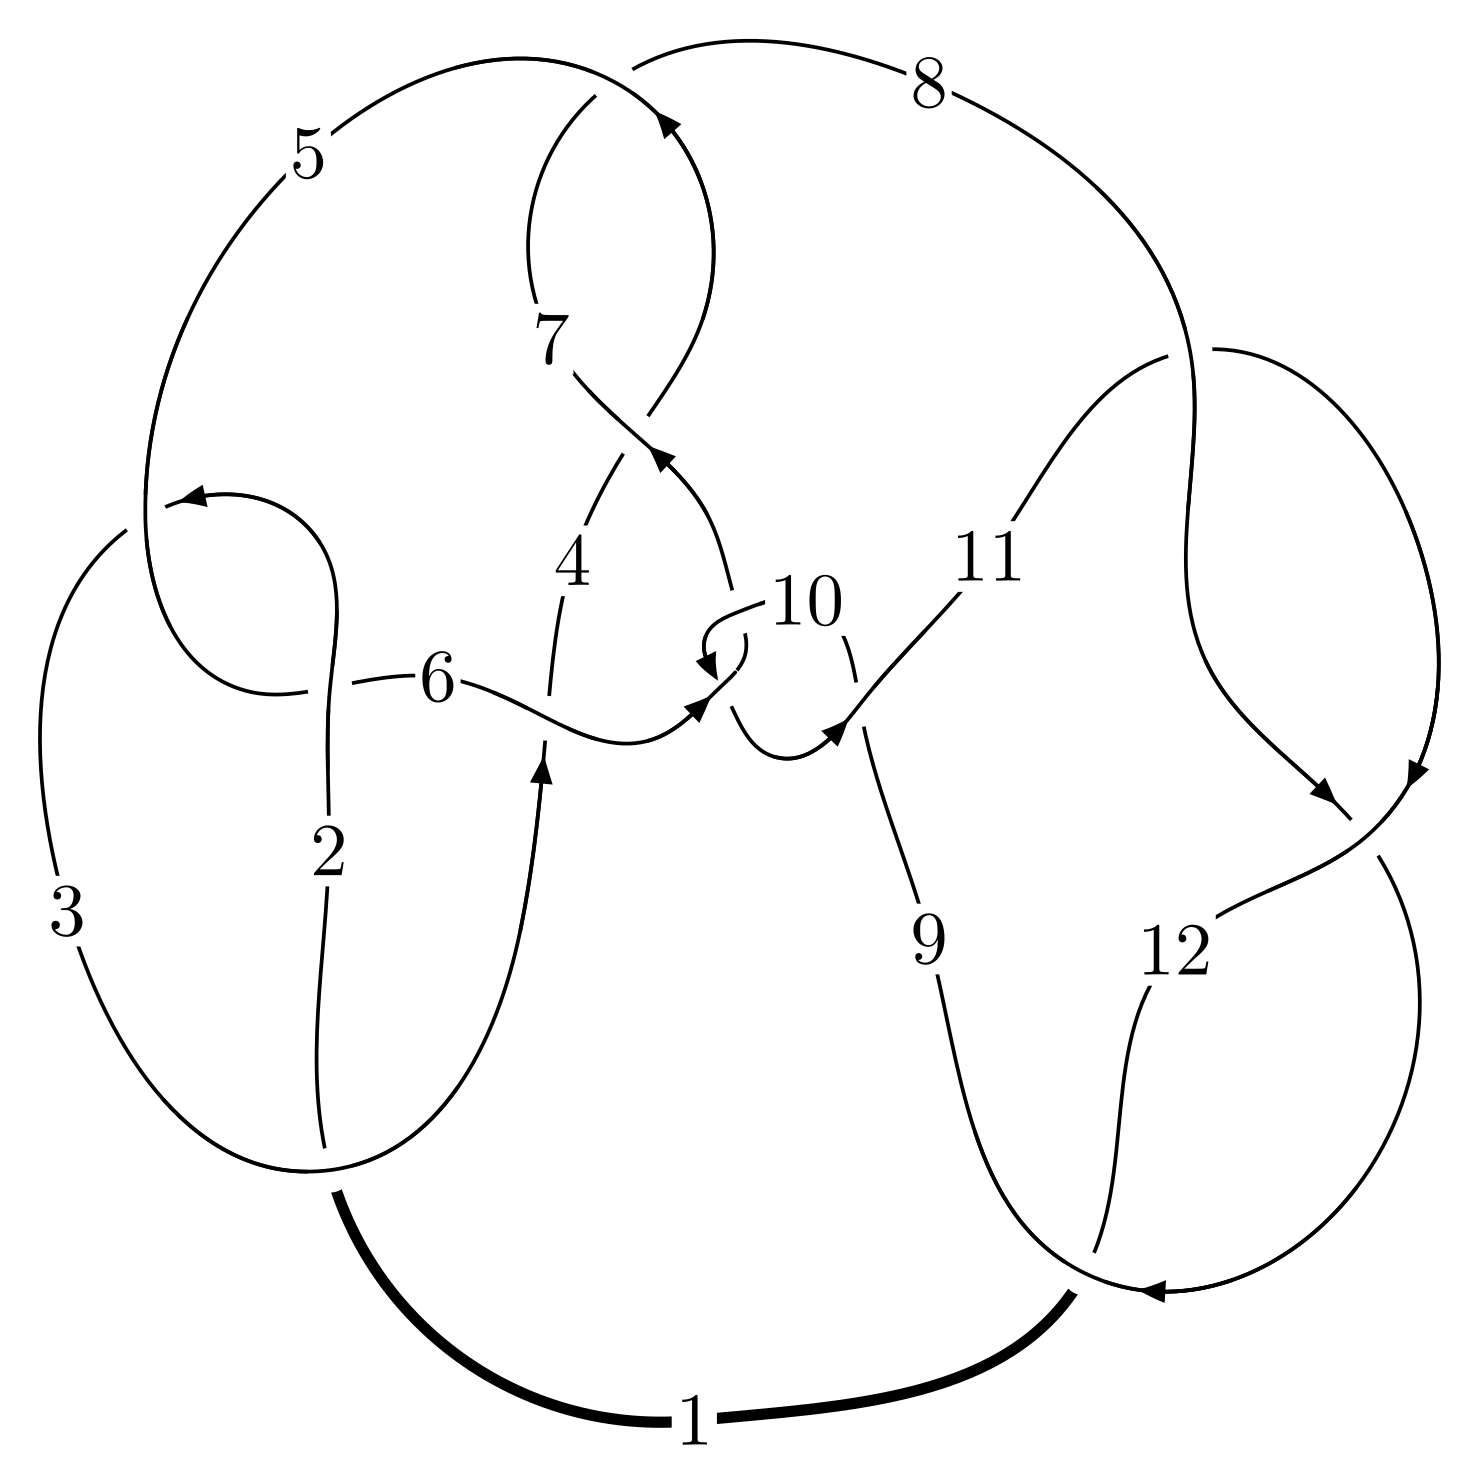
\includegraphics[width=112pt]{../../../GIT/diagram.site/Diagrams/png/2113_12n_0024.png}\\
\ \ \ A knot diagram\footnotemark}&
\allowdisplaybreaks
\textbf{Linearized knot diagam} \\
\cline{2-2}
 &
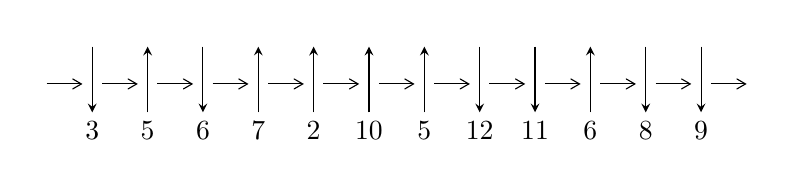
\begin{tikzpicture}[x=20pt, y=17pt]
	% nodes
	\node (C0) at (0, 0) {};
	\node (C1) at (1, 0) {};
	\node (C1U) at (1, +1) {};
	\node (C1D) at (1, -1) {3};

	\node (C2) at (2, 0) {};
	\node (C2U) at (2, +1) {};
	\node (C2D) at (2, -1) {5};

	\node (C3) at (3, 0) {};
	\node (C3U) at (3, +1) {};
	\node (C3D) at (3, -1) {6};

	\node (C4) at (4, 0) {};
	\node (C4U) at (4, +1) {};
	\node (C4D) at (4, -1) {7};

	\node (C5) at (5, 0) {};
	\node (C5U) at (5, +1) {};
	\node (C5D) at (5, -1) {2};

	\node (C6) at (6, 0) {};
	\node (C6U) at (6, +1) {};
	\node (C6D) at (6, -1) {10};

	\node (C7) at (7, 0) {};
	\node (C7U) at (7, +1) {};
	\node (C7D) at (7, -1) {5};

	\node (C8) at (8, 0) {};
	\node (C8U) at (8, +1) {};
	\node (C8D) at (8, -1) {12};

	\node (C9) at (9, 0) {};
	\node (C9U) at (9, +1) {};
	\node (C9D) at (9, -1) {11};

	\node (C10) at (10, 0) {};
	\node (C10U) at (10, +1) {};
	\node (C10D) at (10, -1) {6};

	\node (C11) at (11, 0) {};
	\node (C11U) at (11, +1) {};
	\node (C11D) at (11, -1) {8};

	\node (C12) at (12, 0) {};
	\node (C12U) at (12, +1) {};
	\node (C12D) at (12, -1) {9};
	\node (C13) at (13, 0) {};

	% arrows
	\draw[->,>={angle 60}]
	(C0) edge (C1) (C1) edge (C2) (C2) edge (C3) (C3) edge (C4) (C4) edge (C5) (C5) edge (C6) (C6) edge (C7) (C7) edge (C8) (C8) edge (C9) (C9) edge (C10) (C10) edge (C11) (C11) edge (C12) (C12) edge (C13) ;	\draw[->,>=stealth]
	(C1U) edge (C1D) (C2D) edge (C2U) (C3U) edge (C3D) (C4D) edge (C4U) (C5D) edge (C5U) (C6D) edge (C6U) (C7D) edge (C7U) (C8U) edge (C8D) (C9U) edge (C9D) (C10D) edge (C10U) (C11U) edge (C11D) (C12U) edge (C12D) ;
	\end{tikzpicture} \\
\hhline{~~} \\& 
\textbf{Solving Sequence} \\ \cline{2-2} 
 &
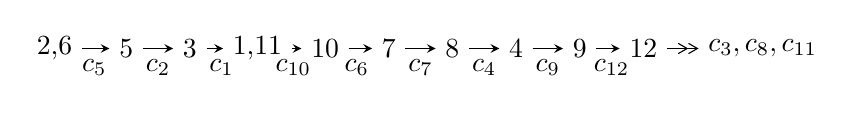
\begin{tikzpicture}[x=23pt, y=7pt]
	% node
	\node (A0) at (-1/8, 0) {2,6};
	\node (A1) at (1, 0) {5};
	\node (A2) at (2, 0) {3};
	\node (A3) at (49/16, 0) {1,11};
	\node (A4) at (33/8, 0) {10};
	\node (A5) at (41/8, 0) {7};
	\node (A6) at (49/8, 0) {8};
	\node (A7) at (57/8, 0) {4};
	\node (A8) at (65/8, 0) {9};
	\node (A9) at (73/8, 0) {12};
	\node (C1) at (1/2, -1) {$c_{5}$};
	\node (C2) at (3/2, -1) {$c_{2}$};
	\node (C3) at (5/2, -1) {$c_{1}$};
	\node (C4) at (29/8, -1) {$c_{10}$};
	\node (C5) at (37/8, -1) {$c_{6}$};
	\node (C6) at (45/8, -1) {$c_{7}$};
	\node (C7) at (53/8, -1) {$c_{4}$};
	\node (C8) at (61/8, -1) {$c_{9}$};
	\node (C9) at (69/8, -1) {$c_{12}$};
	\node (A10) at (11, 0) {$c_{3},c_{8},c_{11}$};

	% edge
	\draw[->,>=stealth]	
	(A0) edge (A1) (A1) edge (A2) (A2) edge (A3) (A3) edge (A4) (A4) edge (A5) (A5) edge (A6) (A6) edge (A7) (A7) edge (A8) (A8) edge (A9) ;
	\draw[->>,>={angle 60}]	
	(A9) edge (A10);
\end{tikzpicture} \\ 

\end{tabular} \\

\footnotetext{
The image of knot diagram is generated by the software ``\textbf{Draw programme}" developed by Andrew Bartholomew(\url{http://www.layer8.co.uk/maths/draw/index.htm\#Running-draw}), where we modified some parts for our purpose(\url{https://github.com/CATsTAILs/LinksPainter}).
}\phantom \\ \newline 
\centering \textbf{Ideals for irreducible components\footnotemark of $X_{\text{par}}$} 
 
\begin{align*}
I^u_{1}&=\langle 
-987290740395 u^{33}-5379029654817 u^{32}+\cdots+837919692176 b-653062691196,\\
\phantom{I^u_{1}}&\phantom{= \langle  }-1563526467031 u^{33}-8197997634981 u^{32}+\cdots+837919692176 a+1275617520034,\\
\phantom{I^u_{1}}&\phantom{= \langle  }u^{34}+6 u^{33}+\cdots+5 u+1\rangle \\
I^u_{2}&=\langle 
- a^3-3 a u+b+3 a+1,\;a^5+a^4 u-2 a^4+2 a^3 u-3 a^3-5 a^2 u+2 a^2-2 a u+4 a+u,\;u^2- u+1\rangle \\
\\
\end{align*}
\raggedright * 2 irreducible components of $\dim_{\mathbb{C}}=0$, with total 44 representations.\\
\footnotetext{All coefficients of polynomials are rational numbers. But the coefficients are sometimes approximated in decimal forms when there is not enough margin.}
\newpage
\renewcommand{\arraystretch}{1}
\centering \section*{I. $I^u_{1}= \langle -9.87\times10^{11} u^{33}-5.38\times10^{12} u^{32}+\cdots+8.38\times10^{11} b-6.53\times10^{11},\;-1.56\times10^{12} u^{33}-8.20\times10^{12} u^{32}+\cdots+8.38\times10^{11} a+1.28\times10^{12},\;u^{34}+6 u^{33}+\cdots+5 u+1 \rangle$}
\flushleft \textbf{(i) Arc colorings}\\
\begin{tabular}{m{7pt} m{180pt} m{7pt} m{180pt} }
\flushright $a_{2}=$&$\begin{pmatrix}0\\u\end{pmatrix}$ \\
\flushright $a_{6}=$&$\begin{pmatrix}1\\0\end{pmatrix}$ \\
\flushright $a_{5}=$&$\begin{pmatrix}1\\u^2\end{pmatrix}$ \\
\flushright $a_{3}=$&$\begin{pmatrix}u\\u^3+u\end{pmatrix}$ \\
\flushright $a_{1}=$&$\begin{pmatrix}u^3\\u^5+u^3+u\end{pmatrix}$ \\
\flushright $a_{11}=$&$\begin{pmatrix}1.86596 u^{33}+9.78375 u^{32}+\cdots+1.06021 u-1.52236\\1.17826 u^{33}+6.41951 u^{32}+\cdots+5.45973 u+0.779386\end{pmatrix}$ \\
\flushright $a_{10}=$&$\begin{pmatrix}0.687698 u^{33}+3.36425 u^{32}+\cdots-4.39952 u-2.30175\\1.17826 u^{33}+6.41951 u^{32}+\cdots+5.45973 u+0.779386\end{pmatrix}$ \\
\flushright $a_{7}=$&$\begin{pmatrix}-1.28785 u^{33}-8.52538 u^{32}+\cdots-21.2336 u-4.29654\\0.361519 u^{33}+2.60589 u^{32}+\cdots+0.591225 u-0.926328\end{pmatrix}$ \\
\flushright $a_{8}=$&$\begin{pmatrix}-1.37658 u^{33}-9.45845 u^{32}+\cdots-25.9217 u-6.02116\\1.27771 u^{33}+6.49148 u^{32}+\cdots+2.68331 u-0.525657\end{pmatrix}$ \\
\flushright $a_{4}=$&$\begin{pmatrix}- u^3\\u^3+u\end{pmatrix}$ \\
\flushright $a_{9}=$&$\begin{pmatrix}0.00960441 u^{33}-1.00925 u^{32}+\cdots-18.8321 u-4.39435\\0.833123 u^{33}+4.09945 u^{32}+\cdots-0.950070 u-1.07697\end{pmatrix}$ \\
\flushright $a_{12}=$&$\begin{pmatrix}-0.818376 u^{33}-6.54935 u^{32}+\cdots-31.6588 u-7.66755\\1.56035 u^{33}+7.49904 u^{32}+\cdots+0.0306098 u-1.66930\end{pmatrix}$\\&\end{tabular}
\flushleft \textbf{(ii) Obstruction class $= -1$}\\~\\
\flushleft \textbf{(iii) Cusp Shapes $= \frac{1379117222209}{837919692176} u^{33}+\frac{1029169729969}{119702813168} u^{32}+\cdots+\frac{2734506517567}{837919692176} u-\frac{434006716289}{104739961522}$}\\~\\
\newpage\renewcommand{\arraystretch}{1}
\flushleft \textbf{(iv) u-Polynomials at the component}\newline \\
\begin{tabular}{m{50pt}|m{274pt}}
Crossings & \hspace{64pt}u-Polynomials at each crossing \\
\hline $$\begin{aligned}c_{1}\end{aligned}$$&$\begin{aligned}
&u^{34}+6 u^{33}+\cdots+17 u+1
\end{aligned}$\\
\hline $$\begin{aligned}c_{2},c_{5}\end{aligned}$$&$\begin{aligned}
&u^{34}+6 u^{33}+\cdots+5 u+1
\end{aligned}$\\
\hline $$\begin{aligned}c_{3}\end{aligned}$$&$\begin{aligned}
&u^{34}-6 u^{33}+\cdots+10043 u+23377
\end{aligned}$\\
\hline $$\begin{aligned}c_{4},c_{7}\end{aligned}$$&$\begin{aligned}
&u^{34}+3 u^{33}+\cdots+4096 u+1024
\end{aligned}$\\
\hline $$\begin{aligned}c_{6},c_{10}\end{aligned}$$&$\begin{aligned}
&u^{34}-3 u^{33}+\cdots-2 u+1
\end{aligned}$\\
\hline $$\begin{aligned}c_{8},c_{11},c_{12}\end{aligned}$$&$\begin{aligned}
&u^{34}-3 u^{33}+\cdots-2 u+1
\end{aligned}$\\
\hline $$\begin{aligned}c_{9}\end{aligned}$$&$\begin{aligned}
&u^{34}+3 u^{33}+\cdots-2 u+1
\end{aligned}$\\
\hline
\end{tabular}\\~\\
\newpage\renewcommand{\arraystretch}{1}
\flushleft \textbf{(v) Riley Polynomials at the component}\newline \\
\begin{tabular}{m{50pt}|m{274pt}}
Crossings & \hspace{64pt}Riley Polynomials at each crossing \\
\hline $$\begin{aligned}c_{1}\end{aligned}$$&$\begin{aligned}
&y^{34}+50 y^{33}+\cdots+17 y+1
\end{aligned}$\\
\hline $$\begin{aligned}c_{2},c_{5}\end{aligned}$$&$\begin{aligned}
&y^{34}+6 y^{33}+\cdots+17 y+1
\end{aligned}$\\
\hline $$\begin{aligned}c_{3}\end{aligned}$$&$\begin{aligned}
&y^{34}+94 y^{33}+\cdots+17344598433 y+546484129
\end{aligned}$\\
\hline $$\begin{aligned}c_{4},c_{7}\end{aligned}$$&$\begin{aligned}
&y^{34}-55 y^{33}+\cdots-6291456 y+1048576
\end{aligned}$\\
\hline $$\begin{aligned}c_{6},c_{10}\end{aligned}$$&$\begin{aligned}
&y^{34}+3 y^{33}+\cdots-2 y+1
\end{aligned}$\\
\hline $$\begin{aligned}c_{8},c_{11},c_{12}\end{aligned}$$&$\begin{aligned}
&y^{34}-25 y^{33}+\cdots-2 y+1
\end{aligned}$\\
\hline $$\begin{aligned}c_{9}\end{aligned}$$&$\begin{aligned}
&y^{34}+59 y^{33}+\cdots+6 y+1
\end{aligned}$\\
\hline
\end{tabular}\\~\\
\newpage\flushleft \textbf{(vi) Complex Volumes and Cusp Shapes}
$$\begin{array}{c|c|c}  
\text{Solutions to }I^u_{1}& \I (\text{vol} + \sqrt{-1}CS) & \text{Cusp shape}\\
 \hline 
\begin{aligned}
u &= \phantom{-}0.460595 + 0.926013 I \\
a &= \phantom{-}1.65664 + 1.65921 I \\
b &= \phantom{-}0.408796 - 0.306002 I\end{aligned}
 & -1.92220 + 2.39604 I & \phantom{-}9.18658 + 7.54131 I \\ \hline\begin{aligned}
u &= \phantom{-}0.460595 - 0.926013 I \\
a &= \phantom{-}1.65664 - 1.65921 I \\
b &= \phantom{-}0.408796 + 0.306002 I\end{aligned}
 & -1.92220 - 2.39604 I & \phantom{-}9.18658 - 7.54131 I \\ \hline\begin{aligned}
u &= \phantom{-}0.916388 + 0.231859 I \\
a &= \phantom{-}0.575411 + 0.072095 I \\
b &= \phantom{-}0.740585 + 0.042237 I\end{aligned}
 & \phantom{-}1.77655 + 0.14759 I & \phantom{-}6.63914 + 0.92800 I \\ \hline\begin{aligned}
u &= \phantom{-}0.916388 - 0.231859 I \\
a &= \phantom{-}0.575411 - 0.072095 I \\
b &= \phantom{-}0.740585 - 0.042237 I\end{aligned}
 & \phantom{-}1.77655 - 0.14759 I & \phantom{-}6.63914 - 0.92800 I \\ \hline\begin{aligned}
u &= -0.139053 + 0.917478 I \\
a &= \phantom{-}0.883284 + 0.335732 I \\
b &= -0.309625 - 1.098890 I\end{aligned}
 & -6.97147 + 2.86372 I & -9.65845 - 4.16249 I \\ \hline\begin{aligned}
u &= -0.139053 - 0.917478 I \\
a &= \phantom{-}0.883284 - 0.335732 I \\
b &= -0.309625 + 1.098890 I\end{aligned}
 & -6.97147 - 2.86372 I & -9.65845 + 4.16249 I \\ \hline\begin{aligned}
u &= \phantom{-}0.615154 + 0.975680 I \\
a &= -0.929833 + 0.597421 I \\
b &= -0.525453 - 0.313759 I\end{aligned}
 & \phantom{-}0.54741 + 2.67952 I & \phantom{-}3.39595 - 1.50494 I \\ \hline\begin{aligned}
u &= \phantom{-}0.615154 - 0.975680 I \\
a &= -0.929833 - 0.597421 I \\
b &= -0.525453 + 0.313759 I\end{aligned}
 & \phantom{-}0.54741 - 2.67952 I & \phantom{-}3.39595 + 1.50494 I \\ \hline\begin{aligned}
u &= \phantom{-}0.429644 + 0.715588 I \\
a &= -0.53311 - 2.00244 I \\
b &= \phantom{-}0.036081 + 0.595902 I\end{aligned}
 & -1.17601 + 1.39012 I & -7.01664 - 5.97525 I \\ \hline\begin{aligned}
u &= \phantom{-}0.429644 - 0.715588 I \\
a &= -0.53311 + 2.00244 I \\
b &= \phantom{-}0.036081 - 0.595902 I\end{aligned}
 & -1.17601 - 1.39012 I & -7.01664 + 5.97525 I\\
 \hline 
 \end{array}$$\newpage$$\begin{array}{c|c|c}  
\text{Solutions to }I^u_{1}& \I (\text{vol} + \sqrt{-1}CS) & \text{Cusp shape}\\
 \hline 
\begin{aligned}
u &= -0.523759 + 0.558320 I \\
a &= -1.97777 - 0.12112 I \\
b &= -0.563128 + 1.220590 I\end{aligned}
 & -5.45470 - 5.60091 I & -2.61064 + 1.17728 I \\ \hline\begin{aligned}
u &= -0.523759 - 0.558320 I \\
a &= -1.97777 + 0.12112 I \\
b &= -0.563128 - 1.220590 I\end{aligned}
 & -5.45470 + 5.60091 I & -2.61064 - 1.17728 I \\ \hline\begin{aligned}
u &= \phantom{-}0.976795 + 0.800627 I \\
a &= -0.742471 + 0.095802 I \\
b &= -0.726847 - 0.193549 I\end{aligned}
 & \phantom{-}1.16029 + 3.25320 I & \phantom{-}4.65048 - 6.79539 I \\ \hline\begin{aligned}
u &= \phantom{-}0.976795 - 0.800627 I \\
a &= -0.742471 - 0.095802 I \\
b &= -0.726847 + 0.193549 I\end{aligned}
 & \phantom{-}1.16029 - 3.25320 I & \phantom{-}4.65048 + 6.79539 I \\ \hline\begin{aligned}
u &= -1.089890 + 0.830630 I \\
a &= \phantom{-}0.725849 + 0.611806 I \\
b &= \phantom{-}1.11344 + 0.97215 I\end{aligned}
 & \phantom{-}9.51601 + 5.95991 I & \phantom{-}0.51921 - 2.93310 I \\ \hline\begin{aligned}
u &= -1.089890 - 0.830630 I \\
a &= \phantom{-}0.725849 - 0.611806 I \\
b &= \phantom{-}1.11344 - 0.97215 I\end{aligned}
 & \phantom{-}9.51601 - 5.95991 I & \phantom{-}0.51921 + 2.93310 I \\ \hline\begin{aligned}
u &= -0.982318 + 0.958357 I \\
a &= \phantom{-}1.53840 + 0.41969 I \\
b &= \phantom{-}1.00540 - 1.12383 I\end{aligned}
 & \phantom{-}8.99044 - 1.80322 I & \phantom{-0.000000 -}0. + 1.42178 I \\ \hline\begin{aligned}
u &= -0.982318 - 0.958357 I \\
a &= \phantom{-}1.53840 - 0.41969 I \\
b &= \phantom{-}1.00540 + 1.12383 I\end{aligned}
 & \phantom{-}8.99044 + 1.80322 I & \phantom{-0.000000 } 0. - 1.42178 I \\ \hline\begin{aligned}
u &= \phantom{-}0.502370 + 1.284930 I \\
a &= \phantom{-}0.386591 - 0.485376 I \\
b &= \phantom{-}0.637032 + 0.537211 I\end{aligned}
 & -1.85905 + 5.40081 I & -1.55683 - 8.82721 I \\ \hline\begin{aligned}
u &= \phantom{-}0.502370 - 1.284930 I \\
a &= \phantom{-}0.386591 + 0.485376 I \\
b &= \phantom{-}0.637032 - 0.537211 I\end{aligned}
 & -1.85905 - 5.40081 I & -1.55683 + 8.82721 I\\
 \hline 
 \end{array}$$\newpage$$\begin{array}{c|c|c}  
\text{Solutions to }I^u_{1}& \I (\text{vol} + \sqrt{-1}CS) & \text{Cusp shape}\\
 \hline 
\begin{aligned}
u &= -0.957231 + 0.999067 I \\
a &= \phantom{-}0.518277 + 0.648716 I \\
b &= \phantom{-}1.11992 + 1.01734 I\end{aligned}
 & \phantom{-}8.85325 - 5.31381 I & \phantom{-0.000000 -}0. + 2.92536 I \\ \hline\begin{aligned}
u &= -0.957231 - 0.999067 I \\
a &= \phantom{-}0.518277 - 0.648716 I \\
b &= \phantom{-}1.11992 - 1.01734 I\end{aligned}
 & \phantom{-}8.85325 + 5.31381 I & \phantom{-0.000000 } 0. - 2.92536 I \\ \hline\begin{aligned}
u &= -1.046170 + 0.937050 I \\
a &= -0.620076 - 0.611485 I \\
b &= -1.11562 - 0.99302 I\end{aligned}
 & \phantom{-}13.38330 + 0.23885 I & \phantom{-}2.96282 + 0. I\phantom{ +0.000000I} \\ \hline\begin{aligned}
u &= -1.046170 - 0.937050 I \\
a &= -0.620076 + 0.611485 I \\
b &= -1.11562 + 0.99302 I\end{aligned}
 & \phantom{-}13.38330 - 0.23885 I & \phantom{-}2.96282 + 0. I\phantom{ +0.000000I} \\ \hline\begin{aligned}
u &= \phantom{-}0.198700 + 0.560261 I \\
a &= -1.17033 - 1.74922 I \\
b &= \phantom{-}0.007937 + 0.744382 I\end{aligned}
 & -1.29654 + 1.36041 I & -5.30238 - 4.63375 I \\ \hline\begin{aligned}
u &= \phantom{-}0.198700 - 0.560261 I \\
a &= -1.17033 + 1.74922 I \\
b &= \phantom{-}0.007937 - 0.744382 I\end{aligned}
 & -1.29654 - 1.36041 I & -5.30238 + 4.63375 I \\ \hline\begin{aligned}
u &= -0.96143 + 1.05476 I \\
a &= -1.50621 - 0.49472 I \\
b &= -1.02274 + 1.10646 I\end{aligned}
 & \phantom{-}12.9727 - 7.5739 I & \phantom{-}2.34047 + 4.26054 I \\ \hline\begin{aligned}
u &= -0.96143 - 1.05476 I \\
a &= -1.50621 + 0.49472 I \\
b &= -1.02274 - 1.10646 I\end{aligned}
 & \phantom{-}12.9727 + 7.5739 I & \phantom{-}2.34047 - 4.26054 I \\ \hline\begin{aligned}
u &= -0.90074 + 1.11269 I \\
a &= \phantom{-}1.50810 + 0.56457 I \\
b &= \phantom{-}1.04148 - 1.09306 I\end{aligned}
 & \phantom{-}8.5560 - 13.1935 I & \phantom{-0.000000 -}0. + 6.90026 I \\ \hline\begin{aligned}
u &= -0.90074 - 1.11269 I \\
a &= \phantom{-}1.50810 - 0.56457 I \\
b &= \phantom{-}1.04148 + 1.09306 I\end{aligned}
 & \phantom{-}8.5560 + 13.1935 I & \phantom{-0.000000 } 0. - 6.90026 I\\
 \hline 
 \end{array}$$\newpage$$\begin{array}{c|c|c}  
\text{Solutions to }I^u_{1}& \I (\text{vol} + \sqrt{-1}CS) & \text{Cusp shape}\\
 \hline 
\begin{aligned}
u &= -0.373509 + 0.310679 I \\
a &= \phantom{-}2.41143 + 0.07043 I \\
b &= \phantom{-}0.482363 - 0.901628 I\end{aligned}
 & -0.05073 - 2.05660 I & \phantom{-}0.17254 + 2.58405 I \\ \hline\begin{aligned}
u &= -0.373509 - 0.310679 I \\
a &= \phantom{-}2.41143 - 0.07043 I \\
b &= \phantom{-}0.482363 + 0.901628 I\end{aligned}
 & -0.05073 + 2.05660 I & \phantom{-}0.17254 - 2.58405 I \\ \hline\begin{aligned}
u &= -0.125550 + 0.377744 I \\
a &= -1.22419 - 1.84916 I \\
b &= -0.829608 - 0.231361 I\end{aligned}
 & -2.61203 - 0.40815 I & -2.95865 - 1.32770 I \\ \hline\begin{aligned}
u &= -0.125550 - 0.377744 I \\
a &= -1.22419 + 1.84916 I \\
b &= -0.829608 + 0.231361 I\end{aligned}
 & -2.61203 + 0.40815 I & -2.95865 + 1.32770 I\\
 \hline 
 \end{array}$$\newpage\newpage\renewcommand{\arraystretch}{1}
\centering \section*{II. $I^u_{2}= \langle - a^3-3 a u+b+3 a+1,\;a^4 u+2 a^3 u+\cdots+2 a^2+4 a,\;u^2- u+1 \rangle$}
\flushleft \textbf{(i) Arc colorings}\\
\begin{tabular}{m{7pt} m{180pt} m{7pt} m{180pt} }
\flushright $a_{2}=$&$\begin{pmatrix}0\\u\end{pmatrix}$ \\
\flushright $a_{6}=$&$\begin{pmatrix}1\\0\end{pmatrix}$ \\
\flushright $a_{5}=$&$\begin{pmatrix}1\\u-1\end{pmatrix}$ \\
\flushright $a_{3}=$&$\begin{pmatrix}u\\u-1\end{pmatrix}$ \\
\flushright $a_{1}=$&$\begin{pmatrix}-1\\0\end{pmatrix}$ \\
\flushright $a_{11}=$&$\begin{pmatrix}a\\a^3+3 a u-3 a-1\end{pmatrix}$ \\
\flushright $a_{10}=$&$\begin{pmatrix}- a^3-3 a u+4 a+1\\a^3+3 a u-3 a-1\end{pmatrix}$ \\
\flushright $a_{7}=$&$\begin{pmatrix}a^4 u- a^4-3 a^2 u- a u+a- u+1\\- a^4 u+3 a^2+a u+u\end{pmatrix}$ \\
\flushright $a_{8}=$&$\begin{pmatrix}a^4 u- a^4-3 a^2 u- a u+a- u+1\\- a^4 u+3 a^2+a u+u\end{pmatrix}$ \\
\flushright $a_{4}=$&$\begin{pmatrix}1\\u-1\end{pmatrix}$ \\
\flushright $a_{9}=$&$\begin{pmatrix}a^4 u+a^4+a^3 u-2 a^3+2 a^2 u-5 a^2-6 a u+2 a- u+2\\2 a^4 u- a^4- a^3 u-3 a^2 u-2 a^2-2 a u+3 a+u\end{pmatrix}$ \\
\flushright $a_{12}=$&$\begin{pmatrix}a^4 u- a^4+a^3-3 a^2 u+a u- a- u\\- a^4 u+a^3 u+3 a^2+a u-2 a\end{pmatrix}$\\&\end{tabular}
\flushleft \textbf{(ii) Obstruction class $= 1$}\\~\\
\flushleft \textbf{(iii) Cusp Shapes $= 6 a^4 u-6 a^4-3 a^3 u-2 a^3-19 a^2 u+5 a^2-11 a u+17 a+4 u+2$}\\~\\
\newpage\renewcommand{\arraystretch}{1}
\flushleft \textbf{(iv) u-Polynomials at the component}\newline \\
\begin{tabular}{m{50pt}|m{274pt}}
Crossings & \hspace{64pt}u-Polynomials at each crossing \\
\hline $$\begin{aligned}c_{1},c_{3},c_{5}\end{aligned}$$&$\begin{aligned}
&(u^2- u+1)^5
\end{aligned}$\\
\hline $$\begin{aligned}c_{2}\end{aligned}$$&$\begin{aligned}
&(u^2+u+1)^5
\end{aligned}$\\
\hline $$\begin{aligned}c_{4},c_{7}\end{aligned}$$&$\begin{aligned}
&u^{10}
\end{aligned}$\\
\hline $$\begin{aligned}c_{6}\end{aligned}$$&$\begin{aligned}
&(u^5- u^4+2 u^3- u^2+u-1)^2
\end{aligned}$\\
\hline $$\begin{aligned}c_{8}\end{aligned}$$&$\begin{aligned}
&(u^5+u^4-2 u^3- u^2+u-1)^2
\end{aligned}$\\
\hline $$\begin{aligned}c_{9}\end{aligned}$$&$\begin{aligned}
&(u^5-3 u^4+4 u^3- u^2- u+1)^2
\end{aligned}$\\
\hline $$\begin{aligned}c_{10}\end{aligned}$$&$\begin{aligned}
&(u^5+u^4+2 u^3+u^2+u+1)^2
\end{aligned}$\\
\hline $$\begin{aligned}c_{11},c_{12}\end{aligned}$$&$\begin{aligned}
&(u^5- u^4-2 u^3+u^2+u+1)^2
\end{aligned}$\\
\hline
\end{tabular}\\~\\
\newpage\renewcommand{\arraystretch}{1}
\flushleft \textbf{(v) Riley Polynomials at the component}\newline \\
\begin{tabular}{m{50pt}|m{274pt}}
Crossings & \hspace{64pt}Riley Polynomials at each crossing \\
\hline $$\begin{aligned}c_{1},c_{2},c_{3}\\c_{5}\end{aligned}$$&$\begin{aligned}
&(y^2+y+1)^5
\end{aligned}$\\
\hline $$\begin{aligned}c_{4},c_{7}\end{aligned}$$&$\begin{aligned}
&y^{10}
\end{aligned}$\\
\hline $$\begin{aligned}c_{6},c_{10}\end{aligned}$$&$\begin{aligned}
&(y^5+3 y^4+4 y^3+y^2- y-1)^2
\end{aligned}$\\
\hline $$\begin{aligned}c_{8},c_{11},c_{12}\end{aligned}$$&$\begin{aligned}
&(y^5-5 y^4+8 y^3-3 y^2- y-1)^2
\end{aligned}$\\
\hline $$\begin{aligned}c_{9}\end{aligned}$$&$\begin{aligned}
&(y^5- y^4+8 y^3-3 y^2+3 y-1)^2
\end{aligned}$\\
\hline
\end{tabular}\\~\\
\newpage\flushleft \textbf{(vi) Complex Volumes and Cusp Shapes}
$$\begin{array}{c|c|c}  
\text{Solutions to }I^u_{2}& \I (\text{vol} + \sqrt{-1}CS) & \text{Cusp shape}\\
 \hline 
\begin{aligned}
u &= \phantom{-}0.500000 + 0.866025 I \\
a &= -0.535003 - 0.266485 I \\
b &= \phantom{-}0.455697 - 1.200150 I\end{aligned}
 & -5.87256 - 2.37095 I & -1.90884 + 0.95814 I \\ \hline\begin{aligned}
u &= \phantom{-}0.500000 + 0.866025 I \\
a &= -1.31030 + 0.92177 I \\
b &= -0.339110 - 0.822375 I\end{aligned}
 & -0.32910 + 3.56046 I & -2.43337 - 7.40396 I \\ \hline\begin{aligned}
u &= \phantom{-}0.500000 + 0.866025 I \\
a &= \phantom{-}1.54372 - 0.52281 I \\
b &= \phantom{-}0.455697 + 1.200150 I\end{aligned}
 & -5.87256 + 6.43072 I & -7.21285 - 8.37016 I \\ \hline\begin{aligned}
u &= \phantom{-}0.500000 + 0.866025 I \\
a &= \phantom{-}0.114093 - 0.334410 I \\
b &= -0.339110 + 0.822375 I\end{aligned}
 & -0.329100 + 0.499304 I & \phantom{-}1.41726 + 0.48644 I \\ \hline\begin{aligned}
u &= \phantom{-}0.500000 + 0.866025 I \\
a &= \phantom{-}1.68749 - 0.66409 I \\
b &= \phantom{-}0.766826\phantom{ +0.000000I}\end{aligned}
 & -2.40108 + 2.02988 I & \phantom{-}0.137791 - 1.258916 I \\ \hline\begin{aligned}
u &= \phantom{-}0.500000 - 0.866025 I \\
a &= -0.535003 + 0.266485 I \\
b &= \phantom{-}0.455697 + 1.200150 I\end{aligned}
 & -5.87256 + 2.37095 I & -1.90884 - 0.95814 I \\ \hline\begin{aligned}
u &= \phantom{-}0.500000 - 0.866025 I \\
a &= -1.31030 - 0.92177 I \\
b &= -0.339110 + 0.822375 I\end{aligned}
 & -0.32910 - 3.56046 I & -2.43337 + 7.40396 I \\ \hline\begin{aligned}
u &= \phantom{-}0.500000 - 0.866025 I \\
a &= \phantom{-}1.54372 + 0.52281 I \\
b &= \phantom{-}0.455697 - 1.200150 I\end{aligned}
 & -5.87256 - 6.43072 I & -7.21285 + 8.37016 I \\ \hline\begin{aligned}
u &= \phantom{-}0.500000 - 0.866025 I \\
a &= \phantom{-}0.114093 + 0.334410 I \\
b &= -0.339110 - 0.822375 I\end{aligned}
 & -0.329100 - 0.499304 I & \phantom{-}1.41726 - 0.48644 I \\ \hline\begin{aligned}
u &= \phantom{-}0.500000 - 0.866025 I \\
a &= \phantom{-}1.68749 + 0.66409 I \\
b &= \phantom{-}0.766826\phantom{ +0.000000I}\end{aligned}
 & -2.40108 - 2.02988 I & \phantom{-}0.137791 + 1.258916 I\\
 \hline 
 \end{array}$$\newpage
\newpage\renewcommand{\arraystretch}{1}
\centering \section*{ III. u-Polynomials}
\begin{tabular}{m{50pt}|m{274pt}}
Crossings & \hspace{64pt}u-Polynomials at each crossing \\
\hline $$\begin{aligned}c_{1}\end{aligned}$$&$\begin{aligned}
&((u^2- u+1)^5)(u^{34}+6 u^{33}+\cdots+17 u+1)
\end{aligned}$\\
\hline $$\begin{aligned}c_{2}\end{aligned}$$&$\begin{aligned}
&((u^2+u+1)^5)(u^{34}+6 u^{33}+\cdots+5 u+1)
\end{aligned}$\\
\hline $$\begin{aligned}c_{3}\end{aligned}$$&$\begin{aligned}
&((u^2- u+1)^5)(u^{34}-6 u^{33}+\cdots+10043 u+23377)
\end{aligned}$\\
\hline $$\begin{aligned}c_{4},c_{7}\end{aligned}$$&$\begin{aligned}
&u^{10}(u^{34}+3 u^{33}+\cdots+4096 u+1024)
\end{aligned}$\\
\hline $$\begin{aligned}c_{5}\end{aligned}$$&$\begin{aligned}
&((u^2- u+1)^5)(u^{34}+6 u^{33}+\cdots+5 u+1)
\end{aligned}$\\
\hline $$\begin{aligned}c_{6}\end{aligned}$$&$\begin{aligned}
&((u^5- u^4+2 u^3- u^2+u-1)^2)(u^{34}-3 u^{33}+\cdots-2 u+1)
\end{aligned}$\\
\hline $$\begin{aligned}c_{8}\end{aligned}$$&$\begin{aligned}
&((u^5+u^4-2 u^3- u^2+u-1)^2)(u^{34}-3 u^{33}+\cdots-2 u+1)
\end{aligned}$\\
\hline $$\begin{aligned}c_{9}\end{aligned}$$&$\begin{aligned}
&((u^5-3 u^4+4 u^3- u^2- u+1)^2)(u^{34}+3 u^{33}+\cdots-2 u+1)
\end{aligned}$\\
\hline $$\begin{aligned}c_{10}\end{aligned}$$&$\begin{aligned}
&((u^5+u^4+2 u^3+u^2+u+1)^2)(u^{34}-3 u^{33}+\cdots-2 u+1)
\end{aligned}$\\
\hline $$\begin{aligned}c_{11},c_{12}\end{aligned}$$&$\begin{aligned}
&((u^5- u^4-2 u^3+u^2+u+1)^2)(u^{34}-3 u^{33}+\cdots-2 u+1)
\end{aligned}$\\
\hline
\end{tabular}\newpage\renewcommand{\arraystretch}{1}
\centering \section*{ IV. Riley Polynomials}
\begin{tabular}{m{50pt}|m{274pt}}
Crossings & \hspace{64pt}Riley Polynomials at each crossing \\
\hline $$\begin{aligned}c_{1}\end{aligned}$$&$\begin{aligned}
&((y^2+y+1)^5)(y^{34}+50 y^{33}+\cdots+17 y+1)
\end{aligned}$\\
\hline $$\begin{aligned}c_{2},c_{5}\end{aligned}$$&$\begin{aligned}
&((y^2+y+1)^5)(y^{34}+6 y^{33}+\cdots+17 y+1)
\end{aligned}$\\
\hline $$\begin{aligned}c_{3}\end{aligned}$$&$\begin{aligned}
&((y^2+y+1)^5)(y^{34}+94 y^{33}+\cdots+1.73446\times10^{10} y+5.46484\times10^{8})
\end{aligned}$\\
\hline $$\begin{aligned}c_{4},c_{7}\end{aligned}$$&$\begin{aligned}
&y^{10}(y^{34}-55 y^{33}+\cdots-6291456 y+1048576)
\end{aligned}$\\
\hline $$\begin{aligned}c_{6},c_{10}\end{aligned}$$&$\begin{aligned}
&((y^5+3 y^4+4 y^3+y^2- y-1)^2)(y^{34}+3 y^{33}+\cdots-2 y+1)
\end{aligned}$\\
\hline $$\begin{aligned}c_{8},c_{11},c_{12}\end{aligned}$$&$\begin{aligned}
&((y^5-5 y^4+8 y^3-3 y^2- y-1)^2)(y^{34}-25 y^{33}+\cdots-2 y+1)
\end{aligned}$\\
\hline $$\begin{aligned}c_{9}\end{aligned}$$&$\begin{aligned}
&((y^5- y^4+8 y^3-3 y^2+3 y-1)^2)(y^{34}+59 y^{33}+\cdots+6 y+1)
\end{aligned}$\\
\hline
\end{tabular}
\vskip 2pc
\end{document}